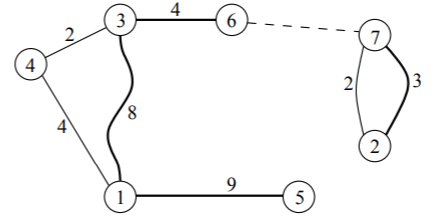
\includegraphics{islands.png}

The $N=7$ bridges in the sample are (1-3), (2-7), (3-4), (4-1), (5-1), (6-3) and (7-2). Note that there are two different bridges connecting islands 2 and 7.
One way that you can achieve maximum walking distance follows:
\begin{itemize}
\item Start on island 5.  
\item Walk the bridge of length 9 to reach island 1.
\item Walk the bridge of length 8 to reach island 3.
\item Walk the bridge of length 4 to reach island 6.
\item Take the ferry from island 6 to island 7.
\item Walk the bridge of length 3 to reach island 2. 
\end{itemize}

By the end you are on island 2 and your total walking distance is 9+8+4+3 = 24. The only island that was not visited is island 4. Note that at the end of the trip described above you can not visit this island any more. More precisely:
\begin{itemize}
\item You are not able to visit it by walking, because there is no bridge connecting island 2 (where you currently stand) and island 4.
\item You are not able to visit it using a ferry, because island 4 is reachable from island 2, where you currently stand. A way to reach it: use the bridge (2-7), then use a ferry you already used to get from island 7 to island 6, then the bridge (6-3), and finally the bridge (3-4).
\end{itemize}